Que faire si nous avons des formules trigonométriques impliquant deux variables, ou plus?
Par exemple,
pour
$(\alpha ; \beta) \in \big( \RRsp \big)^2$ tel que $0 < \alpha + \beta < \frac{\pi}{2}$,
le dessin suivant nous donne
$\cos(\alpha + \beta) = \cos \alpha \cos \beta - \sin \alpha \sin \beta$
et
$\sin(\alpha + \beta) = \cos \alpha \sin \beta + \sin \alpha \cos \beta$.%
%\footnote{
%    Cette démonstration est très utile pour un cours pré universitaire.
%}

\begin{center}
	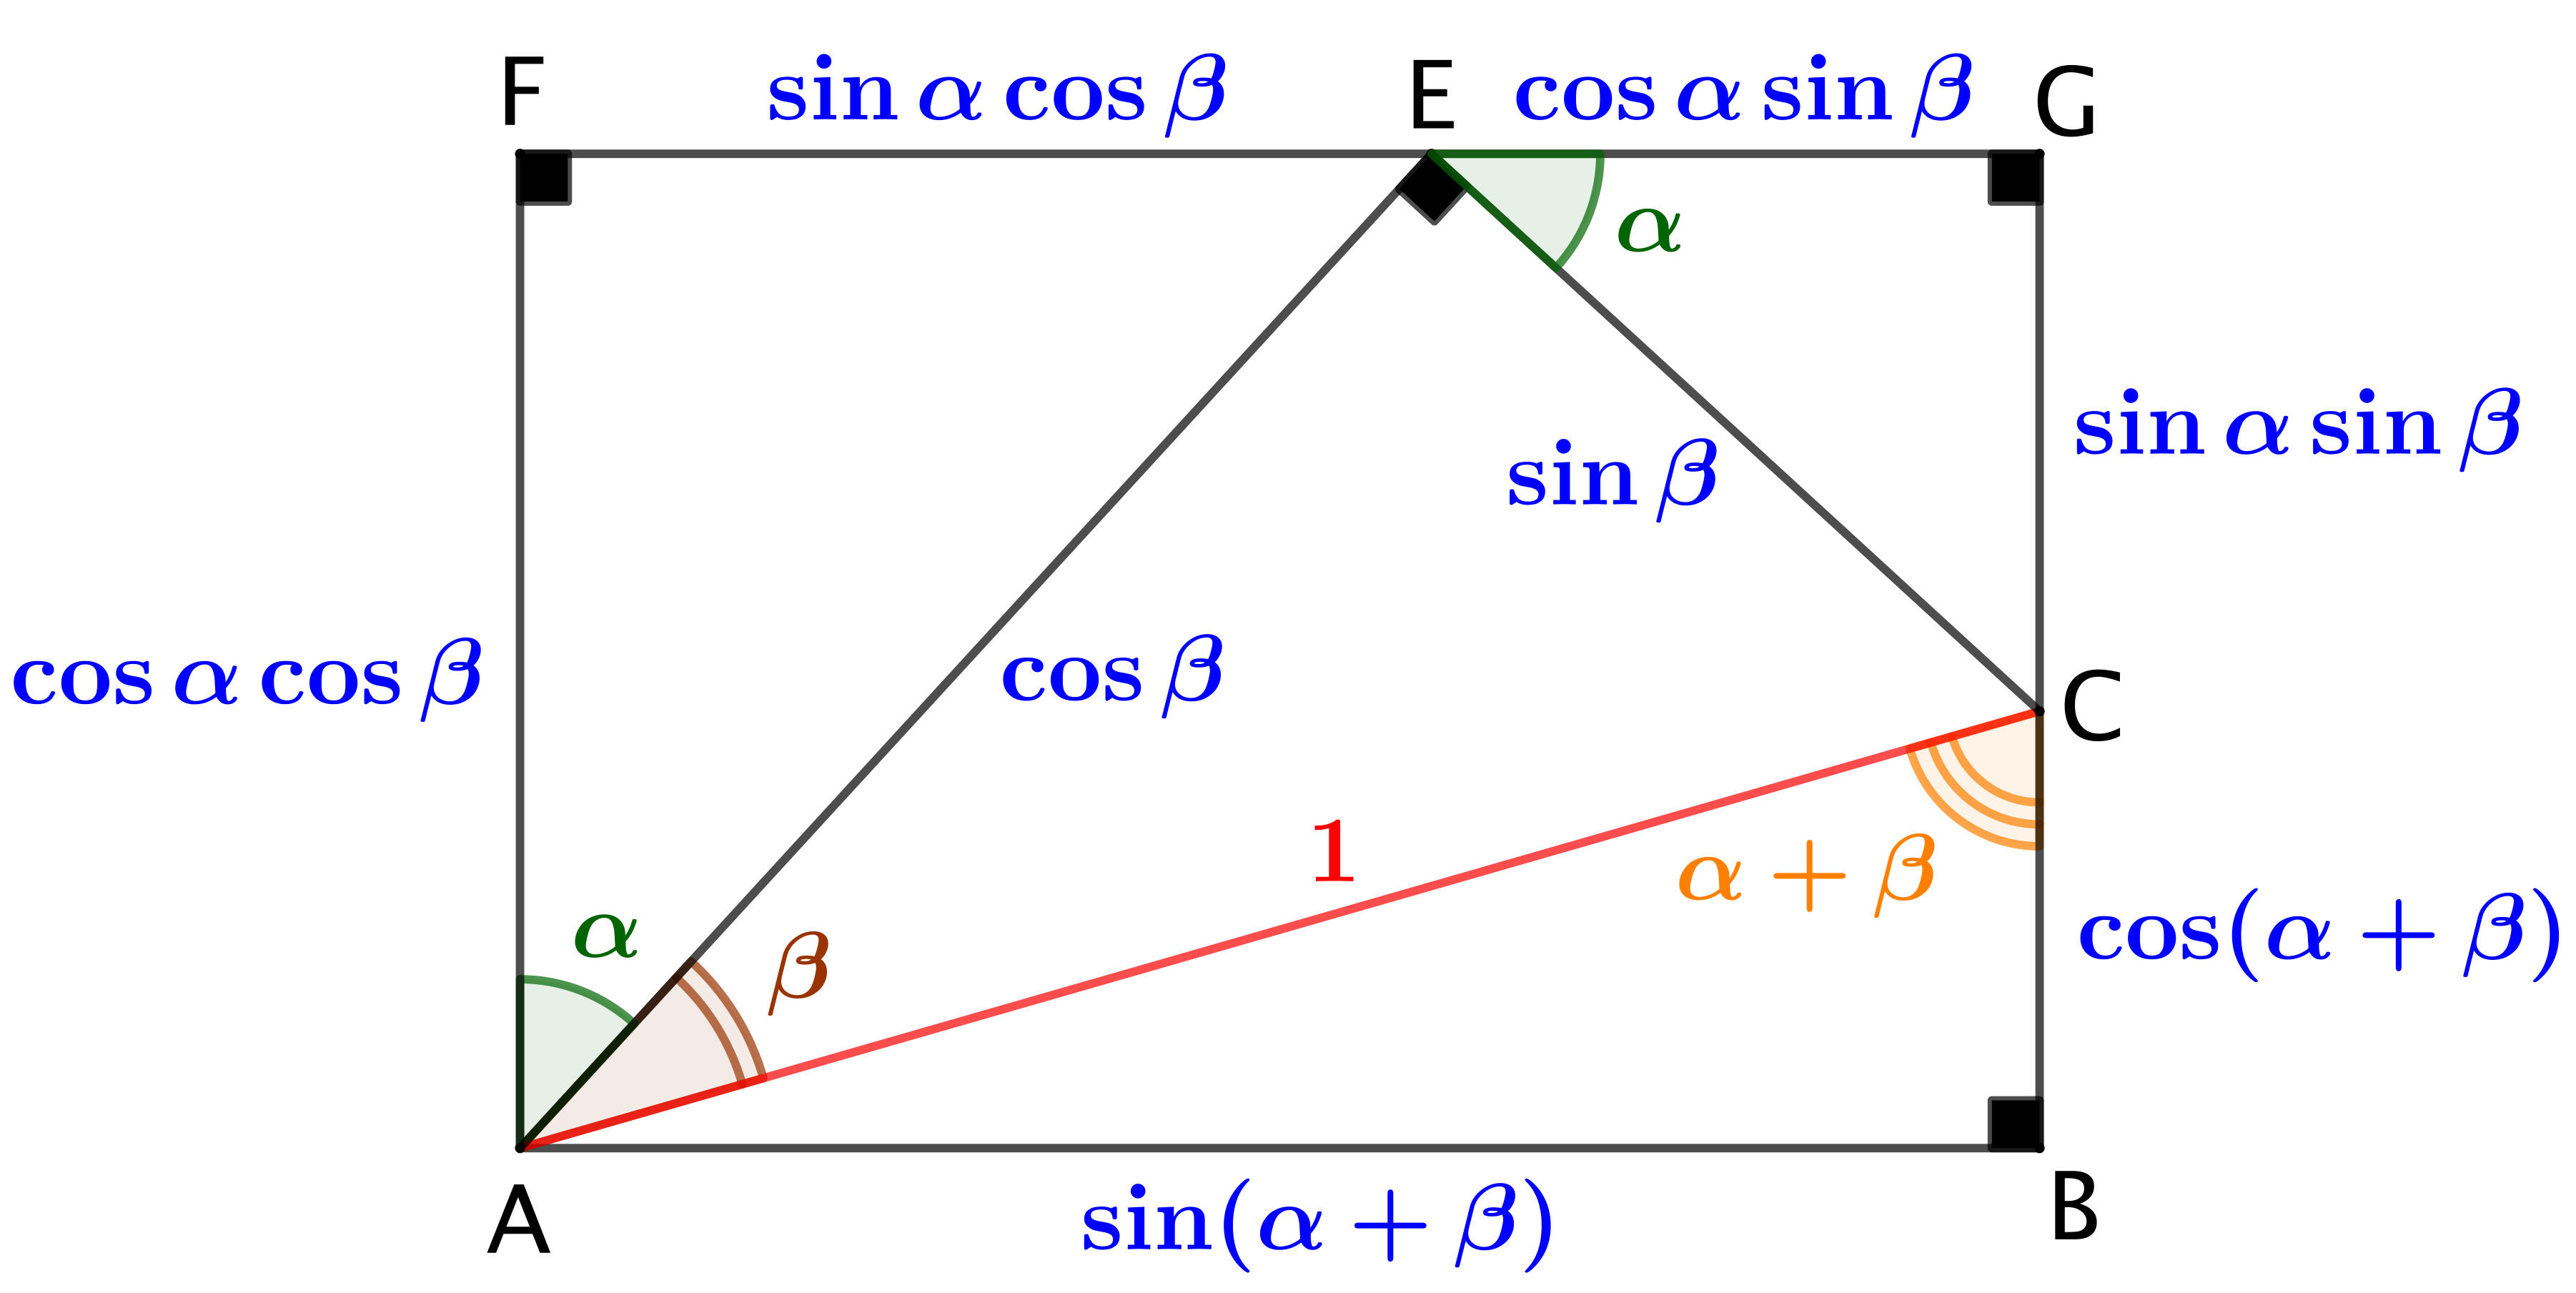
\includegraphics[scale=.7]{add-trigo-formulas.png}
\end{center}

Le \reffact{sep-isolated-zero} ci-dessous, qui généralise le \reffact{isolated-zero}, implique la validité des formules trigonométriques précédentes sur $\CC^2$ tout entier en choisissant
$f_1(\alpha ; \beta) = \cos(\alpha + \beta) - \cos \alpha \cos \beta + \sin \alpha \sin \beta$
et
$f_2(\alpha ; \beta) = \sin(\alpha + \beta) - \cos \alpha \sin \beta - \sin \alpha \cos \beta$.%
\footnote{
    L'ouvert d'annulation est l'intérieur d'un triangle.
}
Nous voilà sauvés!


% ----------- %


\begin{defi}
    Soit $n \in \NNs$.
    %
    Pour $f: \CC^n \rightarrow \CC$
    et
    $k \in \ZintervalC{1}{n}$,
    la \focus{k\ieme\ restriction} de $f$, relative à $(z_1 ; ... ; z_{k-1} ; z_{k+1} ; ... ; z_n) \in \CC^{n-1}$, est définie sur $\CC$ par
    $f_k(z) = f(z_1 ; ... ; z_{k-1} ; z ; z_{k+1} ; ... ; z_n)$.%
	\footnote{
		Avec des abus de notations évidents.
	}
\end{defi}


\begin{defi}
    Soit $n \in \NNs$.
    %
    Une fonction $f: \CC^n \rightarrow \CC$ sera dite \focus{séparablement analytique} sur $\CC^n$,
    si $\forall k \in \ZintervalC{1}{n}$,
    toutes les k\iemes\ restrictions de $f$ sont analytique sur $\CC$.
\end{defi}


\begin{fact} \label{sep-isolated-zero}
    Soient $n \in \NNs$
    et
    $f: \CC^n \rightarrow \CC$ une fonction séparablement analytique.
	Si $f$ s'annule sur un ouvert non vide $\Omega$,
	alors $f$ s'annule sur $\CC^n$. 
\end{fact}


\begin{proof}
	Raisonnons par récurrence sur $n \in \NNs$ pour démontrer la validité de la propriété $\setproba{P}(n)$ définie par
	\emph{\og 
		Pour toute fonction séparablement analytique $f: \CC^n \rightarrow \CC$,
		si $f$ s'annule sur un ouvert non vide $\Omega$,
		alors $f$ s'annule sur $\CC^n$. 
	\fg}\kern2pt.
	%
	\begin{itemize}[label=\small\textbullet]
		\item \textbf{Cas de base.}
		%
		$\setproba{P}(1)$ découle directement du \reffact{isolated-zero}.


		\item \textbf{Hérédité.}
		%
		Supposons $\setproba{P}(n)$ valide pour un naturel $n$ quelconque.
		%
		Soit $f$ une fonction séparablement analytique à $(n + 1)$ variables vérifiant les conditions de la propriété $\setproba{P}(n + 1)$.
		Notons $\Omega$ l'ouvert non vide sur lequel $f$ est nulle.
		%
		Quitte à réduire $\Omega$, on peut supposer que
		$\Omega = \dprod_{k=1}^{n+1} \CdiscO{\alpha_k}{r}$
		avec $r > 0$ et les $\alpha_k$ des complexes fixés.
		%
		\begin{enumerate}
		    \item Pour $\omega \in \CdiscO{\alpha_{n+1}}{r}$ fixé,
		    posons
		    $f_\omega: (z_1 ; ... ; z_n) \in \CC^n \mapsto f(z_1 ; ... ; z_n ; \omega) \in \CC$.
		    Comme $f_\omega$ vérifie les conditions de la propriété $\setproba{P}(n)$, par hypothèse de récurrence,
		    $\forall (z_1 ; ... ; z_n) \in  \CC^n$,
		    $f_\omega(z_1 ; ... ; z_n) = 0$, 
		    soit $f(z_1 ; ... ; z_n ; \omega) = 0$.


		    \item Pour $z_1$ , ... , $z_n$ des complexes quelconques,
		    posons $\ell(z) = f(z_1 ; ... ; z_n ; z)$.
		    Le point précédent montre que $\ell$ vérifie $\setproba{P}(1)$,
		    donc, d'après le cas de base,
		    $\forall z \in \CC$,
		    $\ell(z) = 0$,
		    soit $f(z_1 ; ... ; z_n ; z) = 0$.


		    \item Finalement,
		    $\forall (z_1 ; ... ; z_n ; z) \in  \CC^{n+1}$,
		    $f(z_1 ; ... ; z_n ; z) = 0$.
		    Autrement dit, nous avons déduit la validité de $\setproba{P}(n+1)$ à partir de celle de $\setproba{P}(n)$.
		\end{enumerate}
		
		
		\item \textbf{Conclusion.}
		%
		Par récurrence, $\setproba{P}(n)$ est vraie pour tout naturel non nul $n$.
	\end{itemize}

	\null\vspace{-5.75ex}
\end{proof}


% ----------- %


\begin{example}
    L'implication
    $\big[
        \alpha + \beta + \gamma = \frac{\pi}{2}
        \implies
          \tan \alpha \tan \beta
        + \tan \beta  \tan \gamma
        + \tan \gamma \tan \alpha
        = 1
    \big]$
    est vraie pour 
    $(\alpha ; \beta ; \gamma) \in \big( \RRsp \big)^3$,
    comme le montre le dessin suivant.
    Il est naturel de se demander s'il est possible de partir, plus généralement, de
    $(\alpha ; \beta ; \gamma) \in \big( \CC - \frac{\pi}{2} \ZZ \big)^3$.
    Nous allons voir que c'est le cas.
    %
    \footnote{
    	Pour une fois, la vérification directe est facile, mais cela sort de l'esprit de ce document, et est non généralisable.
		%
		En effet,
		en multipliant par $\cos \alpha \cos \beta \cos \gamma$ l'égalité souhaitée, nous devons démontrer que
		$ \sin \alpha \sin \beta  \cos \gamma
        + \sin \beta  \sin \gamma \cos \alpha
        + \sin \gamma \sin \alpha \cos \beta
        - \cos \alpha \cos \beta  \cos \gamma
        = 0$.
        Dans le terme de gauche, les formules d'addition se cachent de façon ostentatoire.
        Nous obtenons
		$ \sin \alpha \sin(\beta + \gamma)
        - \cos \alpha \cos(\beta + \gamma)$,
        puis
		$ - \cos (\alpha + \beta + \gamma)$,
        soit
		$- \cos (\frac{\pi}{2})$
		qui est bien nul.
    }
    
    \begin{center}
    	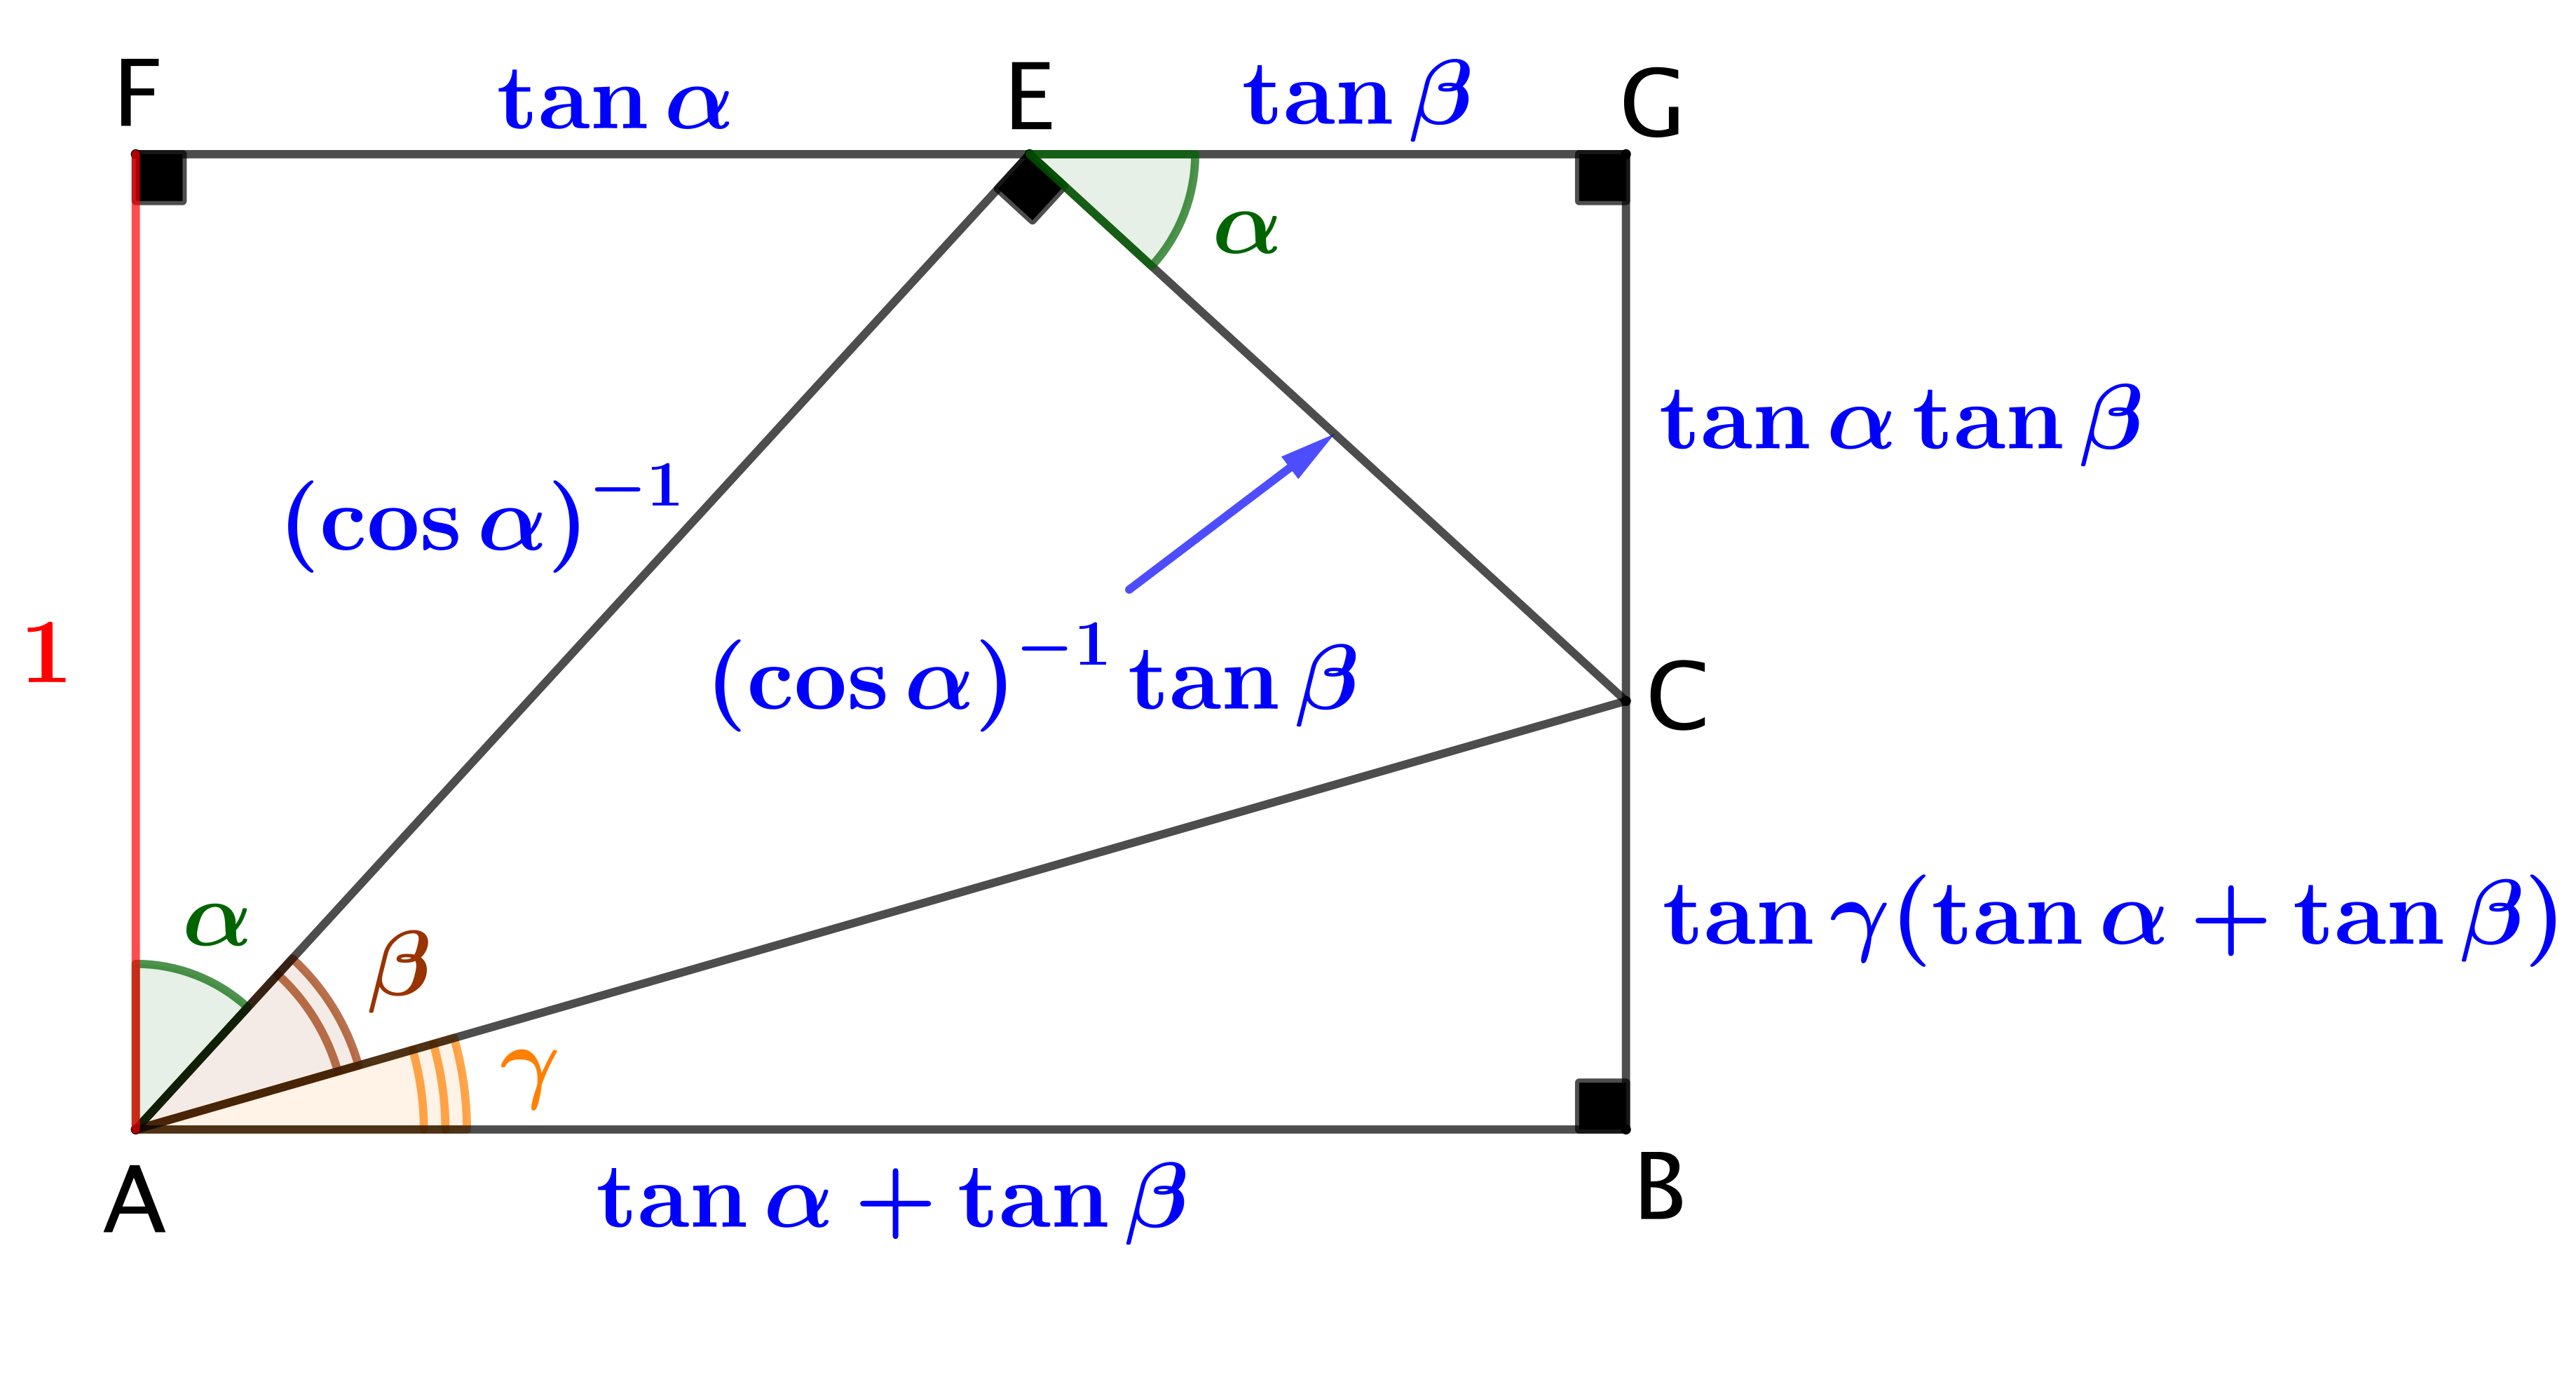
\includegraphics[scale=.75]{sum-tan-prod.png}
    \end{center}
    
    Voici comment arriver à une généralisation pour
    $(\alpha ; \beta ; \gamma) \in \big( \CC - \frac{\pi}{2} \ZZ \big)^3$.
    %
    \begin{itemize}
    	\item XXX


    	\item XXX


    	\item XXX


    	\item XXX


    	\item XXX
    \end{itemize}
\end{example}